\doublespacing
\setlength{\parindent}{1cm}

Scholars and researchers have used different mechanisms to identify ragas. In a system called Tansen, Pandey (Pandey, Mishra, and Ipe, 2003) created a system in which a raga is automatically identified based on Hidden markov model. Pendekar (Pendekar et. al. 2013) were able to identify a raga by segmentation of audio signal via spectral flux and thereby identifying raga by using its pitch frequency. Certain other researchers such as Chelpa (Chelpa, 1991) proposed a fuzzy set theory for generation of alap patterns. Sreedhar et. al. (Sreedhar and Gita, 2009), created a database of ragas and used the scale of the raga performance as a similarity metric using nearest neighbors algorithms. Within a scale, notes are matched with the existing sets of notes in the ragas in the database. The closest raga in the database is given as output for the test raga.
\par
Tzanetakis (Tzanetakis and Cook, 2002) has also proposed various schemes in the English music classification based on their moods and styles of the performer as well as songs genre classification. Clustering is suggested as the classifier (Vaska, 2015). Sentiment analysis of movie review based on naïve Bayes and genetic algorithm is suggested in Govindarajan (Govindarajan, 2013). Since this methodology depends on the likelihood it can be connected to a wide assortment of spaces and results can be utilized as a part of numerous ways (Sharma, 2018). Shetty et. al., (Shetty and Achary, 2009) has identified raga based upon arohana-avorahana pattern on different ragas using neural network technique.
\par
In a 2015 paper (Sharma and Bali, 2015), Sharma and Bali compared several ML classifiers to dataset of music labeled by 4 ragas: Des, Bhupali, Yaman and Todi. The audio performances are converted into .wav extension and chroma features are extracted using MIR toolbox in Matlab. A hop factor of 0.025 second is selected which gives 4719 frames. Then they were able to extract the Vadi swara, also known as the king swara whose magnitude and pitch are relatively greater than notes (swaras). Then they used the WEKA tool which includes a comprehensive collection of machine learning algorithms. The dataset of different ragas is classified using machine learning classifiers in WEKA. Classifiers they used are Random Forest, C4.5, Bayesian network and K-star. After performing comparison of classifiers on ragas, they observed that K-star gives the largest accuracy of 93.38\%, on dataset of ragas followed by the random forest with 92.64\%.
\par
In another work, Kumar et. al. (Kumar et. al. 2014), proposed a method to identify the ragas of an Indian Carnatic music signal. They discuss why this problem is hard due to i) the absence of a fixed frequency for a note, ii) relative scale of notes, iii) oscillations around the note, and iv) improvisations. In this work, they framed the raga classification problem in a non-linear SVM framework using a combination of two kernels that represent the similarities of a music signal using two different features pitch-class profile and n-gram distribution of notes. This differs from the previous pitch-class profile based approaches where the temporal information of notes is ignored. They evaluated the proposed approach on their own raga dataset and CompMusic dataset (CompMusic, 2019) and show an improvement of 10.19\% by combining the information from two features relevant to Indian Carnatic music.
\par
In a recent article, Ale Koretzky (Koretzky, 2019) provides valuable guidance on music signal processing that is helpful for the work that I have to do. Ale addresses the problem of how can we extract vocals out of a mixed track? This is formally known as Audio Source Separation. When we look at a audio source file (,m3 or ,wav), we are visualizing a waveform in the time domain. All we have access to are the amplitude values of the signal over time. While it is possible to extract features like envelopes, RMS values, zero-crossing rate etc., but these features aren’t strong discriminators. To extract vocal content from a mix, we must somehow expose the structure of human speech. This is where the Short-Time Fourier Transform (STFT) comes to our rescue.
\par
\begin{figure}
  \caption{Short Term Fourier Transform of Vocal Audio Sample}
  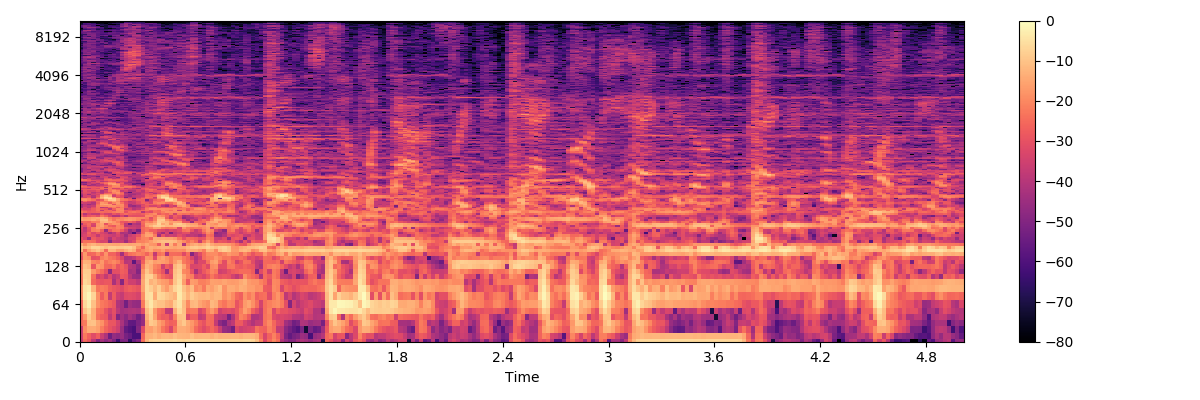
\includegraphics[width=150mm]{vocal-stft.png}
\end{figure}
What the STFT plot shows us are:
\begin{enumerate}[i]
  \item a fundamental frequency (f0) determined by the frequency of the vibration of our vocal cords.
  \par
  The figure below shows Ariana (Koretzky, 2019) is singing in the 300-500 Hz range.
  \item A number of harmonics above f0 following some shape or pattern
  \item no unvoiced speech, which includes consonants like `t', `p,', `k', `s', breaths, etc. \par
  They manifest as short bursts in the high frequency.
\end{enumerate}

The basic idea now is to figure out some sort of mask that when applied (element-wise multiplication) to the magnitude STFT mix gives us an approximate reconstruction pf the magnitude of STFT of the vocals. If this idea works, then we can begin to look at Convolutional Neural Networks (CNN) and what they have been able to achieve on images. Since STFT exhibits spatial patterns (in the time versus frequency space), CNNs should be able to learn from.

\par

Using CNNs on spectral information extracted from librosa to learn patterns has not been explored much in prior work. This is the approach I am going to take in the thesis. My research question becomes:  \par

\textbf{Can CNNs learn and classify ragas based on spectral features represented within chromagrams?}

Before answering this question, it is first important to review what a convolutional neural network is as well as its underlying mechanics for recognizing images in the next chapter.
